\section{Notfallsystem starten}M�chten Sie zu Reparatur- oder Diagnosezwecken einen Client booten, so k�nnen Sie das Notfallsystem �ber Netzwerk booten. Nach dem Booten startet der Client eine Konsole, auf der Sie arbeiten k�nnen. Klicken Sie zum Starten des Notfallsystems auf \textit{"Notfallsystem"} hinter dem Clientnamen.\\
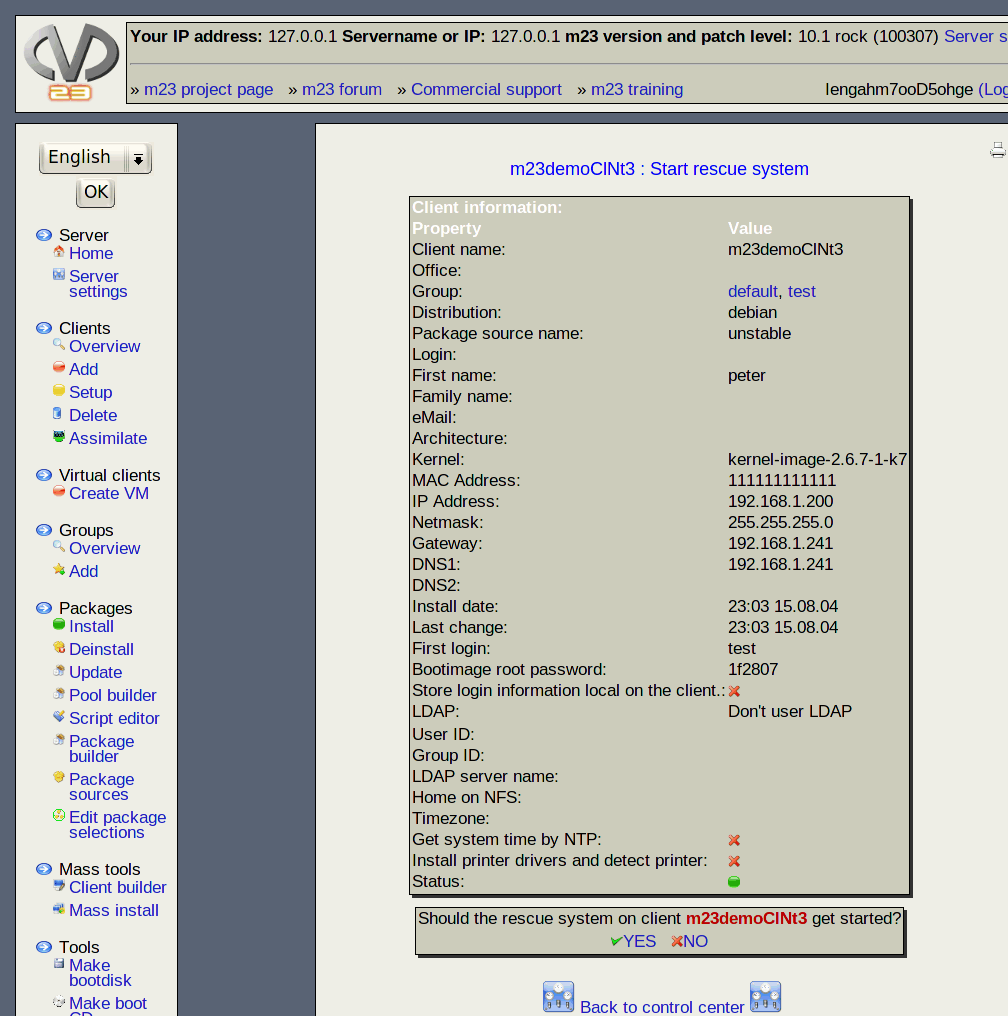
\includegraphics[scale=0.4]{/mdk/doc/manual/screenshots/de/rescue_client.png} \\
\subsection{Hinweis}
Das Notfallsystem wird solange nach dem Booten gestartet, bis Sie den Job \textit{"m23Rescue"} aus der Auftragsliste l�schen. Diese finden Sie, indem Sie auf der Seite \textit{"Clients-�berblick"} auf die Zahl in der Spalte \textit{"Auftr�ge"} klicken.\\
